Alzheimer's Disease (AD) is a devastating neurodegenerative disease that is the most common cause of dementia in persons of age 65 or older. Upon examination, the post-mortem brains of AD patients show significant neuronal dystrophy. Pathologically, AD is characterized by the presence of extracellular deposits of senile plaques and neurofibrillary tangles (NFTs), both of which appear as lesions on stained neuronal tissue under visible-light microscopy (Figure~\ref{fig:AD_tissue_pathology}).

% Biochemistry of the A$beta$ peptide.
In 1985, the amyloid-$\beta$ protein or \abeta\ was identified as the largest component of these plaques.\cite{Masters:1985wb}
% Review paper on AD from science \cite{Hardy:2002dh}
% C.L.Masters etal.,Proc.Natl.Acad.Sci.U.S.A.82,4245 (1985)
% G.G.Glenner,C.W.Wong,Biochem.Biophys.Res. Commun. 120, 885 (1984).
Monomeric \abeta\ is an approximately 4 kDa peptide produced by the intramembrane proteolytic cleavage of a larger protein, the amyloid-$\beta$ precursor protein (APP).\cite{Hardy:2002dh}
% \abeta\ is produced constitutively as part of the normal cellular metabolism.
APP is sequentially processed by the aspartyl proteases $\beta$-secretase and $\gamma$-secretase, producing a pool of \abeta\ peptides of lengths varying from 38 to 43 residues depending on the position of the cleavage by $\gamma$-secretase (Figure~\ref{fig:AD_abeta_app}).\cite{Gandy:2005dd} The peptides spanning residues 1-40 (\abetaforty) or 1-42 (\abetafortytwo) are predominantly found in AD-associated plaques.\cite{Golde:2000vg,Holtzman:2011gi} Although plaques contain different isoforms of the A$\beta$ peptide, \abetafortytwo\ is likely to be the more deleterious form of \abeta. \textit{In vitro}, \abetafortytwo\ displays significantly higher propensity for aggregation than \abetaforty, despite differing by only two amino acids.\cite{Barrow:1992vz,Jarrett:1993ti,ElAgnaf:2000vr} Furthermore, genetic mutations within presenilin 1 and 2 (genes encoding enzymes that cleave APP to produce A$\beta$ peptides) cause an aggressive early-onset form of AD which also lead to an increase in the ratio of \abetafortytwo\ to \abetaforty\ peptides produced.\cite{Hardy:1997tu,KumarSingh:2006kc,Bentahir:2006ih}

% Pathological characterization
\begin{figure}
 \centering
 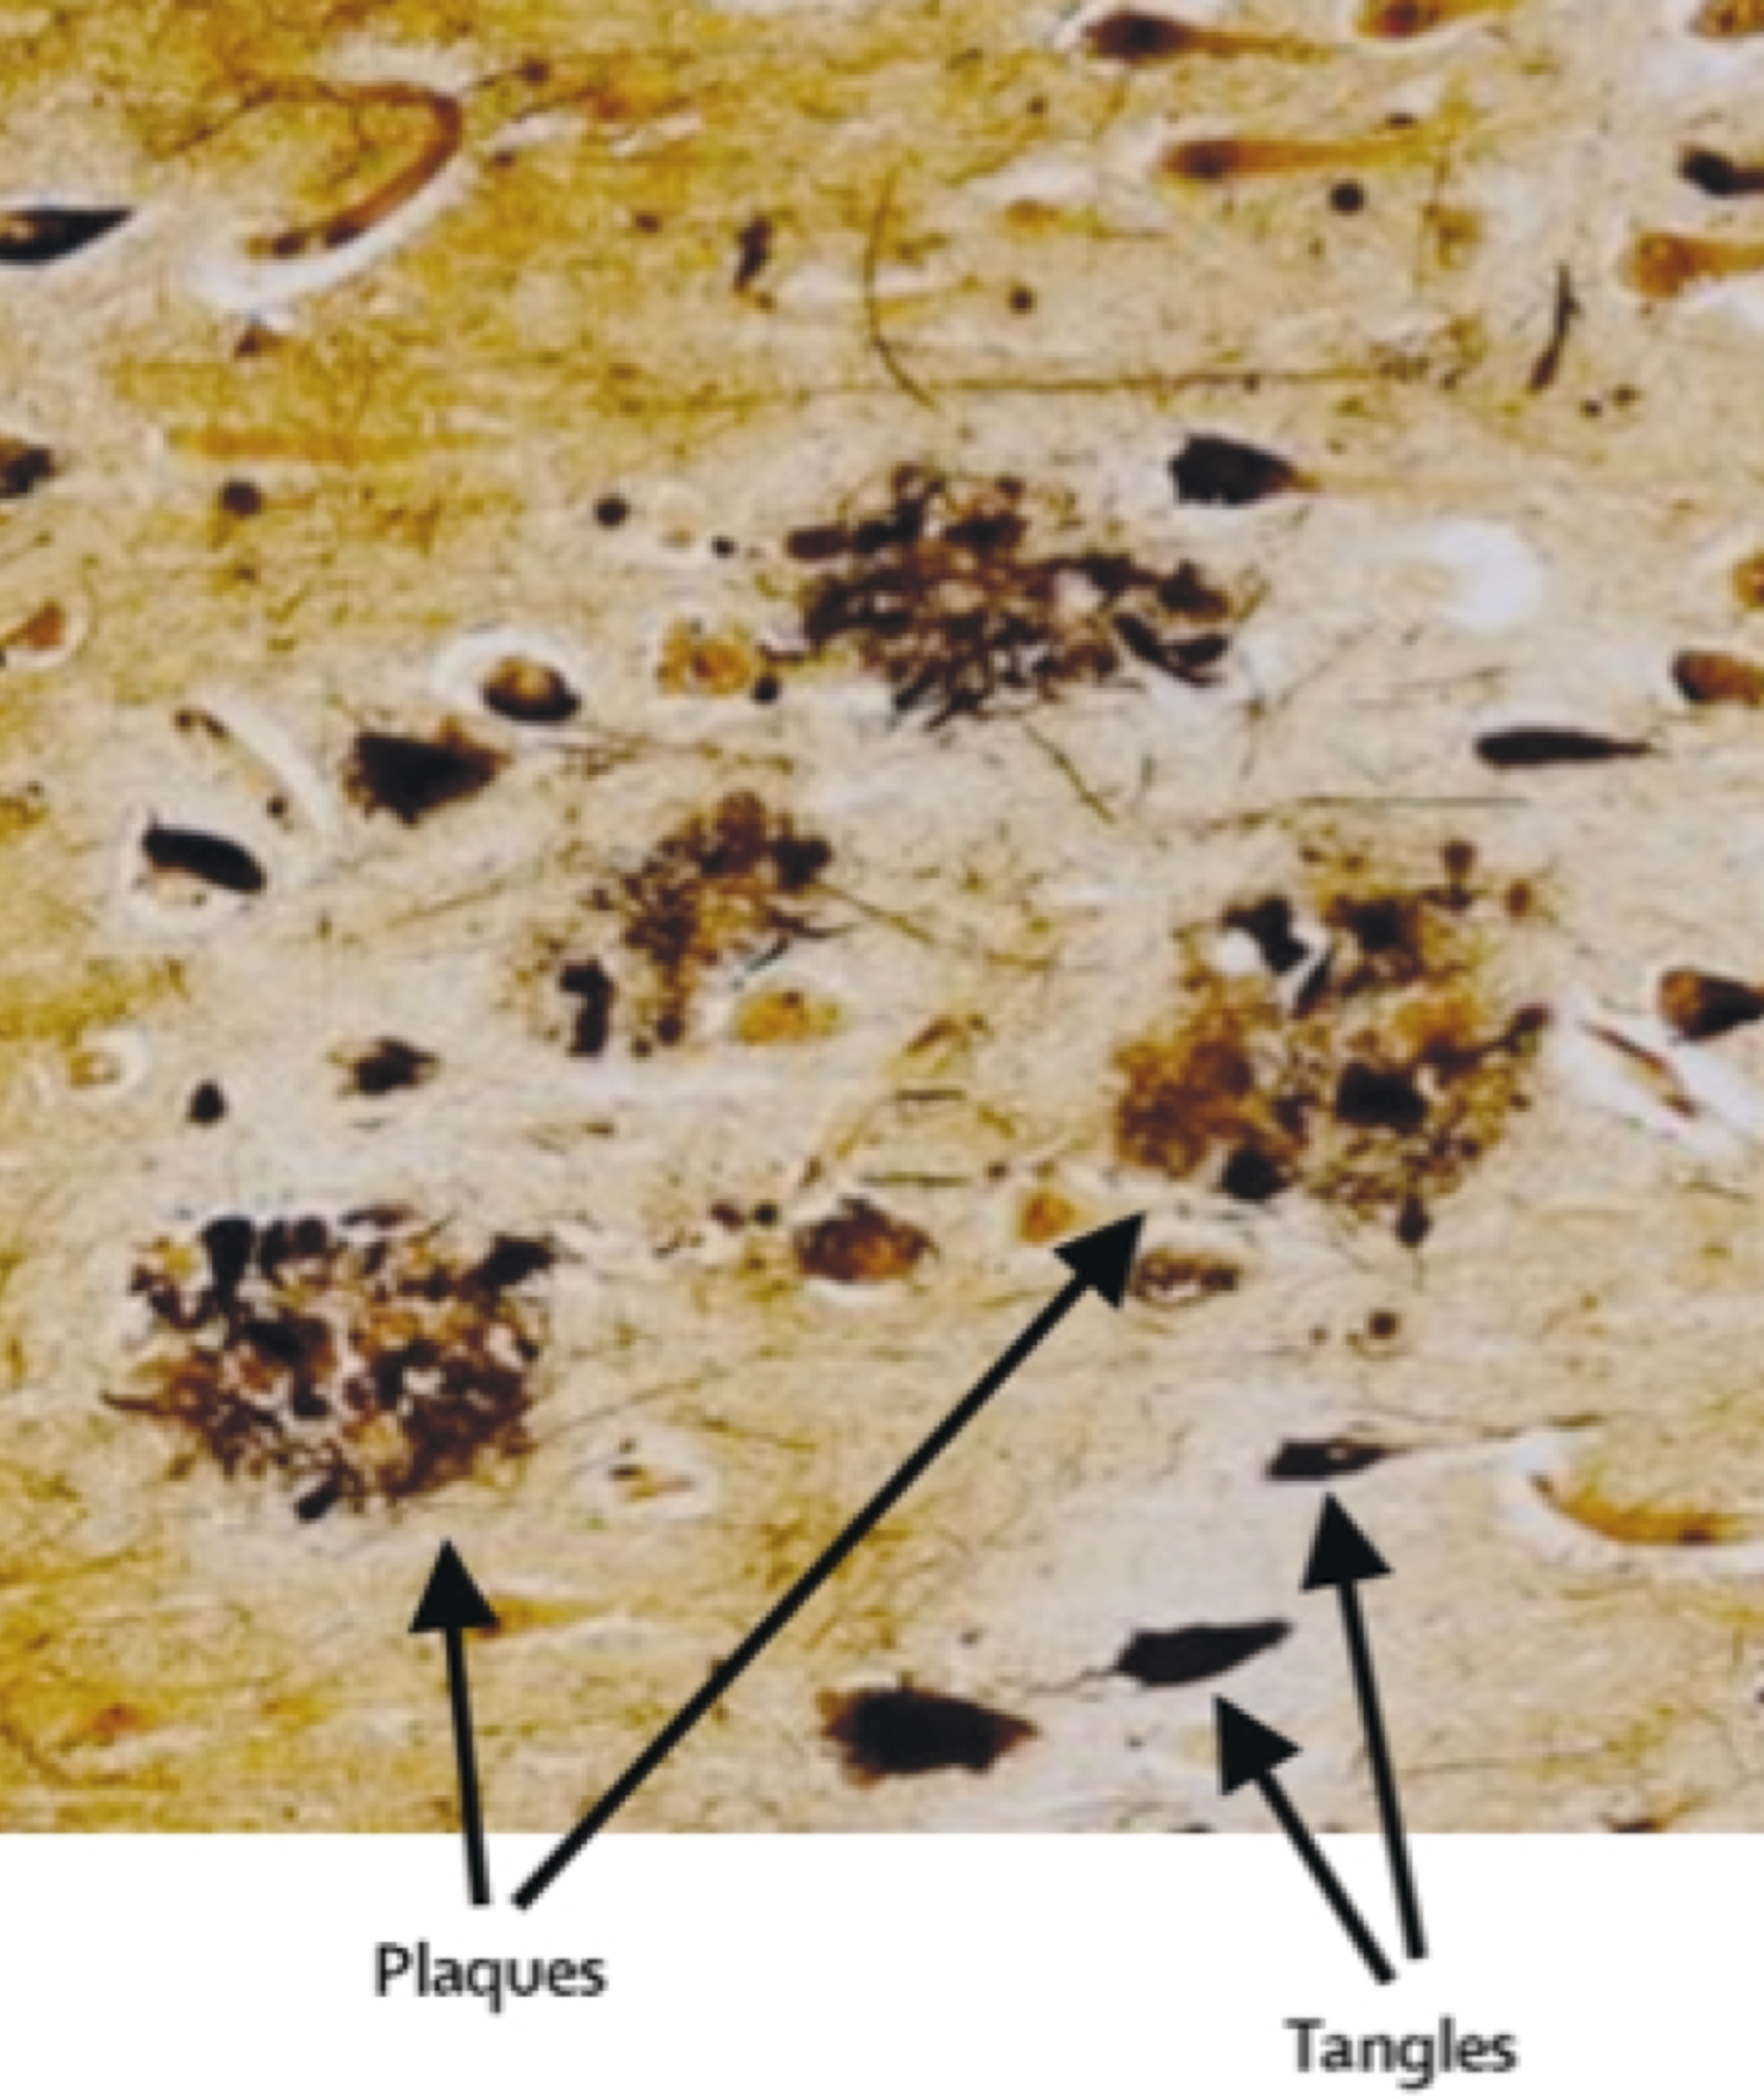
\includegraphics[width=2.5in]{figures/introduction/AD_tissue_pathology.pdf}
 \caption[AD tissue pathology]{Lesions formed from amyloid plaques and NFT tangles in the cerebral cortex tissue of an AD brain. Reprinted from The Lancet, Vol. 368, Kaj Blennow; Mony J de Leon; Henrik Zetterberg, Alzheimer's Disease, 387-403., Copyright 2006, with permission from Elsevier.}
 \label{fig:AD_tissue_pathology}
\end{figure}

\begin{figure}
\centering
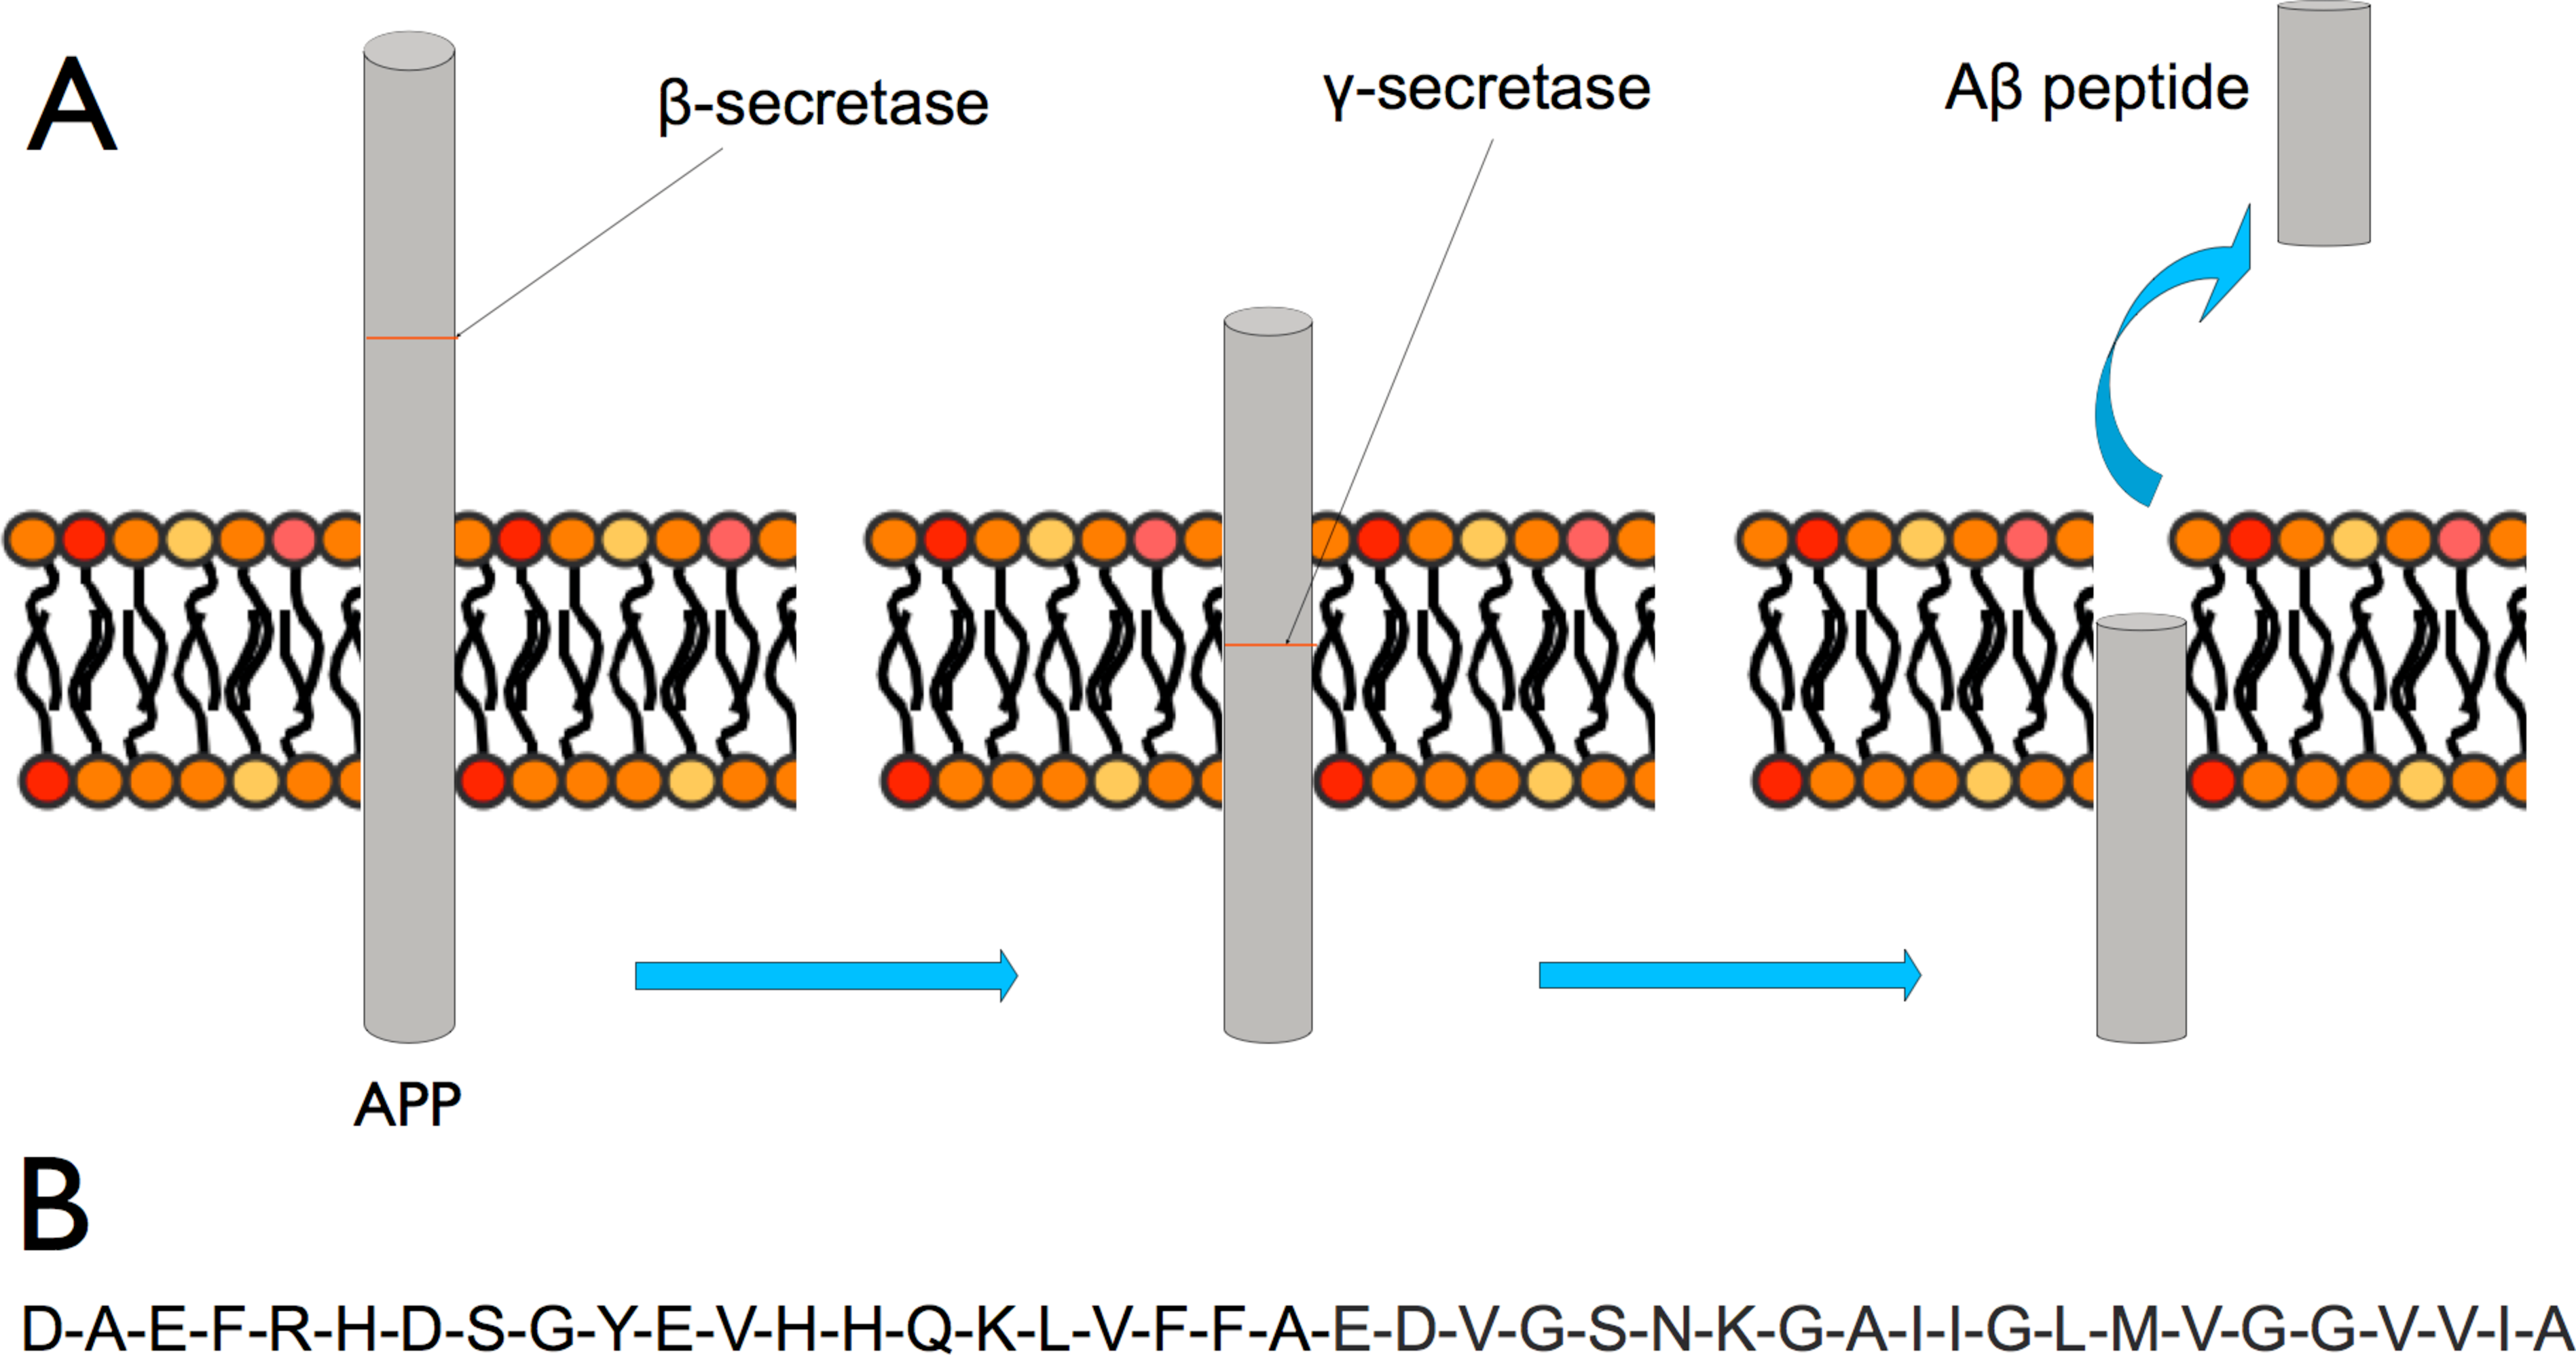
\includegraphics[width=6in]{figures/introduction/AD_abeta_app.pdf}
\caption[APP processing]{A schematic of the production of A$\beta$ via the proteolytic processing of amyloid precursor protein is depicted in (A). The peptide sequence of A$\beta$42 is shown in (B).}
\label{fig:AD_abeta_app}
\end{figure}

% There must be tons of other things that happen in AD .... I’ve made it seem like these oligomers are the only thing that matters.  Perhaps add sentences saying what initiates the disease .. the formation of toxic oligomers. Were the toxicity hypothesis of oligomers for AD have direct evidence from human brain? Look for this. Or was it just pieced together from a bunch of separate animal and cell culture studies? Maybe all of the above.
Although it has been more than one hundred years since Alois Alzheimer first associated the presence of neuronal plaques with the clinical symptoms of Alzheimer's disease, the exact relationship between the two is still under much contention.\cite{Hardy:2002dh} The ubiquitous presence of amyloid plaque deposits found in the brains of deceased dementia patients led to the formulation of the long-standing amyloid cascade hypothesis: the amyloidogenesis of \abeta\ plays a key role in the initiation of AD, which ultimately leads to the clinical symptoms of dementia.\cite{Hardy:2002dh} Genetic evidence provided strong support for the amyloid hypothesis: in those with trisomy 21 (occurring in Down's syndrome), the chromosome responsible for encoding APP, the overproduction of A$\beta$ leads to early-onset of dementia with AD-like plaque load.\cite{Goate:1991kc,LevyLahad:1995vga} Furthermore, in persons with early-onset familial AD, genetic mutations on the APP lead to the production of A$\beta$ peptides with increased aggregation propensities.\cite{Tam:2012vz}
% TODO: Add which mutations -- should I? I have them in a introduction of a chapter.

% Tau protein - Keep discussion brief
In addition to the presence of amyloid plaques, another hallmark of AD is the intracellular deposition of neurofibrillary tangles (NFTs) composed of aggregated hyperphosphorylated forms of the microtubule-associated protein tau.\cite{Ballatore:2007ir} % These tau aggregates have a high $\beta$-sheet content that ultra-structurally appears as paired helical filaments (PHFs) (28, 29).\cite{Holtzman:2011gi}
The role of the tau protein and its interactions with amyloid in the pathogenesis of AD are still being established.\cite{Ittner:2010he} Studies with mouse models currently suggest that the role of NFTs in AD may be downstream to that of \abeta\  because A$\beta$ plaque pathology was not developed in a tau transgenic mouse model, whereas A$\beta$ formation in APP transgenic mice was found to induce hyperphosphorylation of tau, which led to the formation of NFTs.\cite{Gotz:2004dr} 

% A$beta$ and tau review paper -- \cite{Ittner:2010he}
 % More details on evidence which show that NFTs are not likely the causative species.
% I think this detail about abeta aggregation \textit{in vivo} is NICE TO KNOW but could be left out of the thesis.
% The concentration of A$beta$ in the CSF is in the low nanomolar range, but \textit{in vitro} data shows that the critical concentration for aggregation is in the micromolar range. How does it then aggregate in the brain - mechanism of raising the effective concentration.
% \textit{in vitro} models have been useful to screen compound libraries for inhibitors of agregation which may have therapeutic efficacy against AD.

% This was a puzzling aspect of AD which did not fit with the amyloid cascade hypothesis which implicated fibrils as the key cause of toxicity.
A puzzling aspect of AD is that the plaque load in the brain of dementia patients is often not correlated with their disease progression and severity.\cite{Hardy:2002dh,Naslund:2000wf} Instead, multiple lines of evidence indicate that synaptic loss and the severity of cognitive impairment are correlated with the concentration of soluble \abeta\ oligomers in the brain.\cite{Wang:1999fx,McLean:1999ud,Lue:1999vx} For example, oligomers extracted from AD brain can impair synapse structure and function.\cite{Shankar:2008bg}
% Remember to edit this sentence a bit more as I lifted it .. \cite{Tam:2012vz} and references therein.
 Moreover, when injected into the brains of animal models of AD, A$\beta$ oligomers decreased the number of synapses and impaired learning performance.\cite{Lesne:2006gx,Cleary:2005kt,Martins:2007bz,Tam:2012vz} Furthermore, cellullar models of toxicity displayed characteristic symptoms of neurotoxicity that lead to eventual apoptosis upon the addition of A$\beta$ oligomers prepared either \textit{in vitro} or extracted from cell cultures.\cite{Cappai:2007bc,Lambert:1998ve,Walsh:2002p2566,Shankar:2008bg,Walsh:2007fu} Taken together, current experimental evidence indicates that preventing the formation of oligomeric forms of A$\beta$ may be a promising method of treatment for AD.
% Don’t go into the structure here ... it was covered before... 
%A variety of morphologically-different oligomers of \abeta\ have been isolated from the human brain, with the smallest of these oligomers dimeric in size (5).\cite{Roychaudhuri:2009iq}
% Are referred to as ``diffuse'' plaques.\cite{Walsh:2007fu} 
% For example, an oligomeric A? species, termed A??56, purified from the brains of mice in an AD mouse model, was found to disrupt memory functions when administered to young rats.
% Lipids have been used to disassemble A? fibrils into smaller structures, which were seen to be highly active in mice.100 
% Key studies which lead to the toxicity mechanisms. Pull some from\cite{Fandrich:2012kb}

% Other review papers for abeta oligomers \cite{Roychaudhuri:2009iq,Sakono:2010kw}
% SDS- stable low-n oligomers of Ab are the fundamental building blocks of insoluble amyloid deposits and could be the earliest mediators of neuronal dysfunction.\cite{Walsh:2007fu}
% Evidence for the involvement of soluble, non-fibrillar Ab in AD has been gleaned through four distinct experimental approaches that utilize (i) synthetic Ab peptides; (ii) cell culture systems in which APP is over-expressed; (iii) APP transgenic mice; and (iv) human CSF and postmortem brain.
% When Ab is deposited and aggregated in a non–b sheet (nonfibrillar) conformation, it is detected via immunohisto- chemical techniques as “diffuse” plaques (Fig. 1C). REF


% Jarrett JT, Berger EP, Lansbury PT Jr. The carboxy terminus of the beta amyloid protein is critical for the seeding of amyloid formation: implications for the pathogenesis of Alzheimer’s disease. Biochemistry 1993; 32: 4693–97. 
% Walsh DM, Selkoe DJ. Deciphering the molecular basis of memory failure in Alzheimer’s disease. Neuron 2004; 44: 181–93.

% In addition, \abetaforty\ and \abetafortytwo\ also have distinct aggregation pathways \textit{in vitro}: \abetafortytwo\ is found to form a morphologically more diverse population of intermediate oligomers than \abetaforty.\cite{Bitan:2003ut} 

% What about mice studies? LOOK AT DAVIS THESIS FOR MORE REFERENCES THERE IN SUPPORT OF ABETA42

% Soluble oligomers - structure? toxicity on cells? rats? mouse?
% What kind of an effect do they have? Synaptic toxicity.

% Take a look at how Lemkul covers this section and transitions to it.
% In this section, I will provide an overview of some of the challenges to overcome when developing a small molecule therapeutic for Alzheimer's disease. Furthermore, using this information, I will motivate why inositol is an exciting avenue to explore.
% Briefly mention non-small molecule putative therapies which also acts via amyloid inhibition. The focus of this thesis will be on small-molecule amyloid inhibition.
% Amyloid inhibition as a treatment for Alzheimer's disease and related amyloid disorders. 
% Talk about how important it is to develop drugs for these amyloid disorders 
